% -*- coding : utf8 -*-
%; whizzy -pdf
\documentclass[nodefaultblocks]{beamer}
\usepackage{beamerthemesplit}

\usepackage[T1]{fontenc}
\usepackage[utf8]{inputenc}
\usepackage{lmodern}
\usepackage{graphicx}

\usepackage{pgf,pgfarrows,pgfnodes}
\usepackage{tikz}
\usepackage{alltt}
%\usetikzlibrary{shapes}
%\usetikzlibrary{arrows,snakes,backgrounds}
%\usepackage{xy} 
%\xyoption{all} 


\newcommand{\ocaml}{OCaml}
\newcommand{\metapost}{Metapost}


\def \ybox #1{{\mbox { \strut #1}}}

\usetheme{Madrid}
\beamertemplatenavigationsymbolsempty
\date{August 30, 2009}

\definecolor{yel}{rgb}{.9,.8,.4}
\definecolor{mygray}{rgb}{0.85,0.85,0.85}

\def \ebox #1{\colorbox{yel}{\mbox {\strut #1}}}
\def \gbox #1{\colorbox{mygray}{\mbox {\strut #1}}}
\def \goldbox #1{\colorbox{mygold}{\mbox {\strut #1}}}
\def \magbox #1{\colorbox{mymagenta}{\mbox {\strut #1}}}
\definecolor{mymagenta}{rgb}{1,0,1}
\definecolor{mygold}{rgb}{1,.7,0.1}

\definecolor{darkgray}{gray}{0.5}
\definecolor{mygreen}{rgb}{0,0.5,0}
\definecolor{myblue}{rgb}{0.1,0.1,0.8}
\definecolor{royalblue}{rgb}{0.282,0.463,1.0}
\def \blue #1{{\color{myblue} #1}}
\def \green #1{{\color{mygreen} #1}}
\def \red #1{{\color{red} #1}}
\def \gray #1{{\color{darkgray} #1}}
\def \toto{\only<-2>{white}\only<3->{black}}

\newcommand{\colornodeboxstroke}[4]{%
{\color{#1}\pgfnodebox{#2}[fill]{#3}{#4}{3pt}{3pt}}%
\pgfnodebox{#2}[stroke]{#3}{#4}{3pt}{3pt}}



\newcommand{\colornodebox}[4]{%
{\color{#1}\pgfnodebox{#2}[fill]{#3}{#4}{2pt}{2pt}}%
\pgfnodebox{#2}[virtual]{#3}{#4}{2pt}{2pt}}

\newcommand{\fleche}[3]{%
\begin{pgfscope}\pgfsetlinewidth{1.2pt}%
\pgfsetendarrow{\pgfarrowtriangle{3pt}}%
{\color{#1}\pgfnodeconnline{#2}{#3}}\end{pgfscope}}


\definecolor{lred}{rgb}{1,0.8,0.6}
\definecolor{lightgray}{rgb}{0.7,0.7,0.7}
\definecolor{lightgreen}{rgb}{0.6,1,0.8}
\definecolor{darkgreen}{rgb}{0,0.6,0}
\definecolor{royalblue}{rgb}{0.25,0.41,0.88}

\title{Mlpost - A scientific drawing library}
\author[Bardou,\hspace{0.05em}  
        Bobot, \hspace{0.05em}  
        Filliâtre, \hspace{0.05em}  
        Kanig, \hspace{0.05em}  
        Lescuyer]{ Romain Bardou, François Bobot, Jean-Christophe Filliâtre \\
         \alert{Johannes Kanig}, Stéphane Lescuyer}
\institute[]{LRI, Proval INRIA Saclay - Île-de-France}

\begin{document}

\begin{frame}
  \maketitle
\end{frame}

\begin{frame}[fragile]\frametitle{Motivation}
  how to make nice pictures
  \begin{itemize}
  \item with embedded \LaTeX\ snippets
  \item scripted in a nice language
  \item possibly resulting from computations
  \end{itemize}
  \begin{overprint}
    \onslide<+>
  \begin{center}
  \bigskip
  \includegraphics{fibtree.pdf}
  \end{center}
    \onslide<+>
    \medskip
    \begin{center}
      \medskip
     \begin{alltt}
  open \alert{Mlpost}

  let texint n = tex (sprintf "$F_\{%d\}$" n)

  let rec fib = function
    | 0 | 1 as n -> leaf (texint n)
    | n -> node (texint n) [fib (n-1); fib (n-2)]

  let fibtree = draw (fib 6)

      \end{alltt}
    \end{center}
    \onslide<+>
    \medskip
    Alternatives: 
    \begin{itemize}
    \item dia, xfig
    \item PGF/Tikz 
    \item Metapost
    \item functional metapost
    \end{itemize}
  \end{overprint}
\end{frame}

\begin{frame}{Our contribution : Mlpost = \ocaml\ + \metapost}

  \begin{columns}
    \column{0.5\textwidth}
  A stub of basic \metapost\ features
  \begin{itemize}
    \item embedded \LaTeX\ snippets
      \item Bézier paths
  \end{itemize}

  \column{0.5\textwidth}
  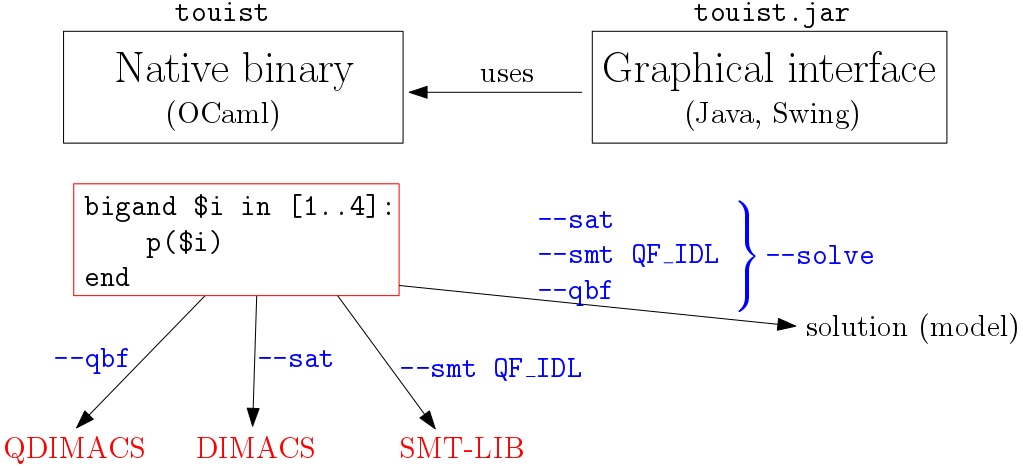
\includegraphics[width=\textwidth]{../../papers/jfla2009/architecture.mps}
  \end{columns}
  \bigskip
  Additional features
  \begin{itemize}
    \item High-level libraries: boxes, trees, diagrams, radars, function plots
  \item persistence (allows sharing) 
  \item uses optional/labeled arguments massively
  \end{itemize}

\end{frame}

\begin{frame}
  \frametitle{Two backends}
  \begin{center}
  \includegraphics{archi_backend}
  \end{center}
\end{frame}

\begin{frame}
\frametitle{Example 1: for a math lecture}
\begin{center}
  \includegraphics[width=0.6\textwidth]{../../papers/jfla2009/ford.mps} 
\end{center}
\end{frame}

\begin{frame}[fragile]
\frametitle{Example 2: The histogram library}
\begin{columns}
  \column{0.6\textwidth}
\begin{verbatim}
  Hist.stack 
    ~fill:[lightred;lightblue;
           lightyellow;lightgreen]
    [[4.;5.;5.;]; 
     [8.;3.;1.]; 
     [2.;8.;1.;4.]]  
\end{verbatim}
  \column{0.4\textwidth}
\begin{center}
  \includegraphics{hist}
\end{center}

\end{columns}

\end{frame}

\begin{frame}[fragile]
\frametitle{Example 3: Easy diagrams using boxes}
\begin{columns}
  \column{0.75\textwidth}
\small
\begin{verbatim}



let diag =
  let rt s = rect (tex s) in
  let a = rt "A" and b = rt "B" and c = rt "C" in
  let ab = round_rect (hbox [a;b]) in
  let v = vbox [ab;c] in
  let arrow x y = box_arrow (sub x v) (sub y v) in
  draw v ++ arrow a b ++ arrow ab c 
\end{verbatim}
\column{0.25\textwidth}
\includegraphics{diag}
\end{columns}

\end{frame}
\begin{frame}
\frametitle{Example 4: From a previous talk}

\begin{center}
\includegraphics[width=\textwidth]{gray_f0}
\end{center}
\end{frame}

\begin{frame}
  \frametitle{Example 5: from a PhD thesis}
  \includegraphics[width=0.6\textwidth]{../../papers/jfla2009/figures_flo/chrono2_1.mps}
  \includegraphics[width=0.4\textwidth]{../../papers/jfla2009/figures_flo/automate_jfla.mps}
\end{frame}


\begin{frame}\frametitle{Conclusion}

Mlpost is freely distributed at

\begin{center}
  \url{http://mlpost.lri.fr}
\end{center}

There is a debian package (currently in \tt{testing})

\end{frame}


\end{document}

